\section{Preliminary}
\label{sec:preliminary}

% \begin{figure}[h]
% 	\centering
% 	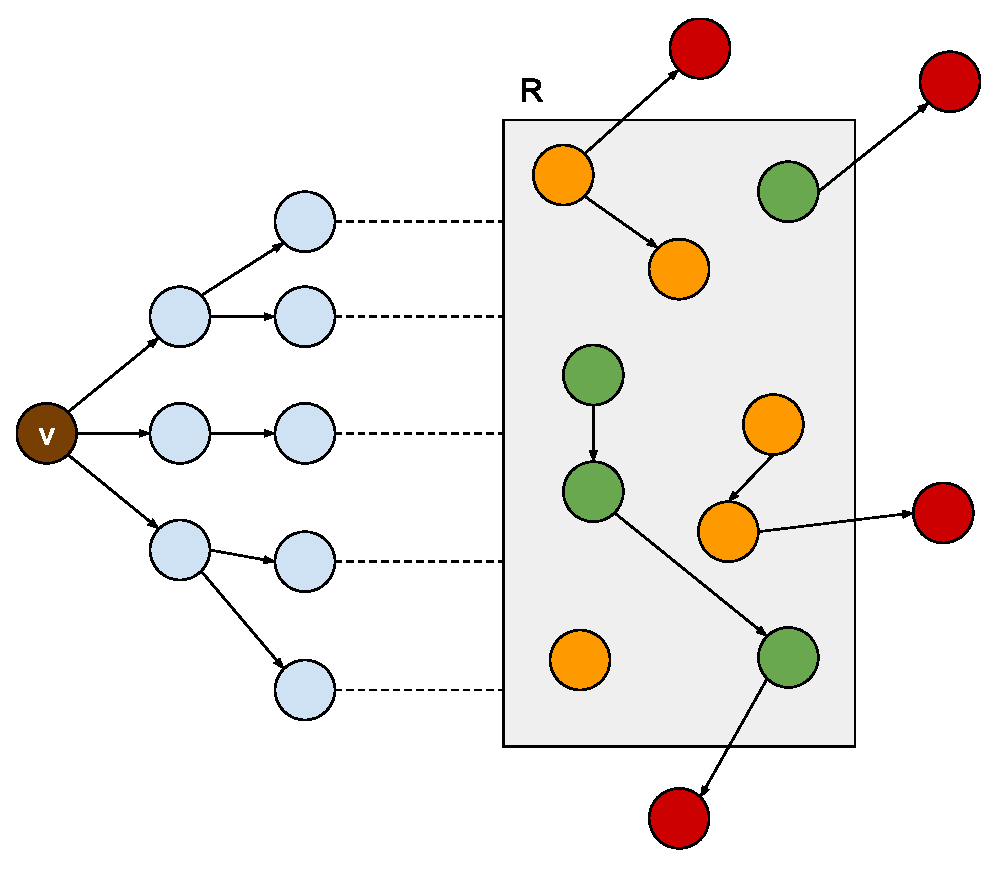
\includegraphics[width=0.44\textwidth]{images/a_social_graph.eps}
% 	\caption{A social graph showing friend-friend connections and also the region of interest}
% 	\label{fig:socio-spatial-graph}
% \end{figure}

{\bf GeoSocial Graph Data.} It is a graph contains people, real spatial venues and relationships among these entities. We use the following to model the GeoSocial graph. It is a directed graph $G=(V,E,S)$ consisting of (1) a set of vertices $V$ representing people and spatial venues; (2) a set of directed edges, $E\subset V\times V$ with weights. If $(u,v)\in E$, there exists one edge from vertex $u$ to $v$, which means the two entities possess a real-life connection. The connection can be {\Friendof} or {\Rate}. The weights of the edge indicates which how strong the two entities are connected. The shorter a distance, the stronger it is; (3) a function $S$ defined on $V$ that decides spatial attribute of a given vertex. $S(v)$ returns spatial property of $v$ (denoted as $v.spatial$), generally for venues, and the value will be null when $v$ brings no spatial attribute, generally for people. $S(v)$ can be a geometrical a point, line, or polygon. For ease of presentation, we assume that a spatial attribute of spatial vertex is represented by a point.

\textbf{Path and Shortest Path.} A path is a sequence of vertices and edges that are distinct from one another. A path is denoted as $p =$ ($v_1$, $e_1$,..., $v_{n-1}$, $e_{n-1}$, $v_n$) where $v_i\neq v_j~and~e_i\neq e_j (i\neq j)$. Length of $p$ is denoted as $L(p) = \sum\limits_{i = 1}^{n-1}w(e_i)$. This path starts from vertex $v_1$ to $v_n$. In a GeoSocial graph $G$, given a source vertex $u$ and destination vertex $v$, there can be multiple paths between them. $Paths(u,v) = \{p|p = (u,e_1,..., v)\}$ is to represent the set of all paths that start from $u$ and end at $v$. Then we can have the shortest path between $u$ and $v$ defined as follows. $ShortestPath(u,v)$ is a path that has the shortest $L(p)$ where $p\in Paths(u,v)$.

\textbf{Socially k-Nearest Neighbors with GeoSpatial Range Filter({\query}).} Based on GeoSpatial range filter and social distance, we can define such a new meaningful query(we use $v\sqsubset R$ if a vertex $v$ is located in a region $R$):
\begin{defn}
	{\query}(v,R,k) = $\widetilde{V}$ where $\widetilde{V}\subset V_{\sqsubset R}$, $\widetilde{V}$ has n elements, $V_{\sqsubset R} = \{u~|~u\sqsubset R\}$ and $\forall w_1\in \widetilde{V}$, $\forall w_2$ $\in$ $V_{\sqsubset R}$ $-$ $\widetilde{V}$, $ShortestPath(v,w_1)$ $\leqslant ShortestPath(v,w_2)$.
	%For a set $V_{\sqsubset R}$ consists of all the spatial venues that are located in $R$, {\query}(v,R,k) = \{$u_1$,..., $u_k$\} where $u_i\sqsubset R$ and 
\end{defn}

{\query} gets as input a source vertex $v$, a spatial region $R$ and number of returned venues $K$ and returns a set that consists of $K$ venues that are located in $R$ and can be reachable from $v$ through $k$ shortest path among all located venues.
%\textbf{Shortest Path or Socially closest.} In $G$, there can be multiple paths between two vertices $u$ and $v$. $Paths(u,v) = \{p|p = (u,e_1,..., v)\}$ is to represent the set of all paths that start from $u$ and end at $v$. Shortest path between $u$ and $v$ is a path that has the shortest $L(p)$ where $p\in Paths(u,v)$, denoted as $ShortestPath(u,v)$. As we are in a geospatial graph world, shortest path between two people nodes is an objective way to indicate the strength of their relationship. Similarly shortest path between a person node and a spatial node (generally a venue) is a numerical way to represent the person's preference strength of that venue.

%\textbf{Shortest path between vertex and spatial region.} Given a vertex $v$ and a spatial region $R$, there exist many shortest paths from $v$ to $U$, where $U$ is the set of all vertices in $R$. RangeReachPaths($G$, $v$, $R$, $K$) returns $K$ shortest paths among all shortest paths 
\iffalse
\begin{eqnarray*}
  	(P_1..P_K) \ni P_i = ShortestPath(v, u_i) | u_i \in U\ and\\
  	P_i(v, u_i) \neq P_j(v, u_j) \leftrightarrow u_i \neq u_j
\end{eqnarray*}


Given a graph $G(V, E)$ where,

\quad$V \rightarrow set\ of\ vertices$

\quad$E \rightarrow set\ of\ edges$

$Vs \subset V$ have spatial attributes; i.e. $\forall v \in Vs \Leftrightarrow v.spatial$ attribute exists\\


\textbf{RangeReachPaths S(G, v, R, K):} an ordered list of K shortest paths starting from v that reach a region R in graph G, where R is a spatial range predicate. Let's abbreviate this as {\rrp}(G, v, R, K).

\textbf{Path, P(u, w):} A set of vertices along the way from u to w \(\Rightarrow w\ is\ reachable\ from\ u\)

\quad${P(u, w) \in S(v, R) \Leftrightarrow}$

\quad\quad{u = v and}

\quad\quad${w \in Vs}$ and

\quad\quad{w.spatial lies in region R}\\

\fi

See Figure \ref{fig:begin-example} to understand the problem better. When a query {\query}(Terry, $R$, 2) is issued, \{G, F, H, I, K\} are all the vertices that are located in the region $R$. Aim of the query is to find two venues socially closest to Terry among \{G, F, H, I, K\}. Assume that F and G have shorter distance to Terry than the other vertices \{H, I, K (not reachable)\}, then G and F will be result of such {\query} query.

%See Figure \ref{fig:begin-example} to understand the problem better. Let `Bob' be the source vertex, v and R be the region of interest. A, B, ... K vertices have spatial attributes like latitude and longitude information. \{A, B, C, D, E, J\} vertices fall outside the region and so are not returned by {\rrp}. Vertex K falls inside R but cannot be reached from v, so are not returned by {\rrp}. \{F, H, G, I\} vertices satisfy both these conditions as they fall inside the region and are also reachable from v. Therefore, {\rrp} may return shortest paths to them. These paths with rich social information about the relationship with v, can be fed into a recommendation system which can rank them. \textit{RangeReachPaths in a geospatial graph produces K venues in a region ranked by the social distances to the source vertex.}

There are two state of the art solutions namely {\socialfirst} and {\spatialfirst}, which take a disjointed approach filtering first by social and then spatial or spatial and then social constraints respectively. 

\textbf{SocialFirst algorithm.} Such approach uses the social constraint of K shortest distances first and then checks for spatial predicate. State of the art single source shortest path algorithm traverses the graph greedily from the source vertex until K closest vertices to source in the query region are found. During traversal, every vertex is checked if it falls in the region and the algorithm stops once K vertices are found. As this is a greedy approach which finds vertices in the increasing order of their distances to the source, the first K vertices found in the region are the closest ones.

%{\rrp} is compared to state of the art existing solutions namely SocialFirst and SpatialFirst which take a disjointed approach filtering first by social and then spatial or spatial and then social constraints respectively. \textbf{SocialFirst algorithm}, uses the social constraint of K shortest distances first and then checks for spatial predicate. State of the art single source shortest path algorithm traverses the graph greedily from the source vertex until K closest vertices to source in the query region are found. During traversal, every vertex is checked if it falls in the region and the algorithm stops once K vertices are found. As this is a greedy approach which finds vertices in the increasing order of their distances to the source, the first K vertices found in the region are the closest ones.

\textbf{SpatialFirst algorithm. } Vertices in the given region R are first filtered and shortest distances to each are found. After sorting them in ascending by distance from the source, first K are picked. For filtering the vertices in R, R-Tree is used and for finding the shortest distance from the source vertex to each vertex in the region, A* with landmark algorithm~\cite{AC2005} is used. This algorithm finds the shortest path between two vertices using precomputed landmarks like explained in Algorithm \ref{alg2}. The closest K vertices based on distances returned by A* with landmark algorithm are picked. 

% In the preprocessing stage for this algorithm:
% \begin{itemize}
% 	\item A r-tree indexed by spatial vertices of the graph is created
% 	\item Shortest distances to each landmark are stored. This is used by A* with landmark's heuristic function
% \end{itemize}


% Algorithm \ref{alg5} outlines SpatialFirst algorithm, where state of the art spatial index, r-tree, to filter vertices in R was used on Line~\ref{alg:rtree}. The best K based on distances returned by A* with landmark algorithm are picked.

% \begin{algorithm}[t]
% \caption{SpatialFirst Algorithm}
% \begin{scriptsize}
% \label{alg5}
% \begin{algorithmic}[1]
% \Function{SpatialFirst}{G, s, R, K}
%   \State F $\gets$ RTree.filter(R) \label{alg:rtree}
%   \For{v $\gets$ F}
% 	  \State distances[v] $\gets$ \Call{A*\_with\_landmark}{s, v}
%   \EndFor
%   \State Order vertices in F using distances
%   \State \Return first K vertices in F
% \EndFunction
% \end{algorithmic}
% \end{scriptsize}
% \end{algorithm}